\chapter{METODOLOGI PENELITIAN}
%\section{Tempat dan Jadwal Kegiatan Penelitian}
%Dalam melaksanakan sebuah penelitian, perencanaan waktu merupakan komponen kritis yang memastikan alur penelitian dapat berjalan dengan terstruktur dan sistematis. Gambar \ref{fig:jadwal-penelitian} menyajikan jadwal penelitian yang telah dirancang untuk penelitian ini. Jadwal tersebut mencakup rentang waktu mulai dari September 2023 hingga April 2024 dan menguraikan berbagai kegiatan yang akan dilakukan selama periode tersebut. Selanjutnya, penelitian ini akan dilaksanakan di Laboratorium Komputer, Institut Teknologi Sumatera.
%
%\begin{figure}[h!]
%    \centering
%    \includegraphics[width=1\textwidth]{figures/ch03/Timeline-2.png}
%    \caption{Jadwal Penelitian}
%    \label{fig:jadwal-penelitian}
%\end{figure}


\section{Alur Penelitian}
Penelitian ini terdapat enam tahapan utama yang ditunjukkan pada Gambar \ref{fig:diagram alir}. Langkah awal yang dilakukan adalah melakukan identifikasi masalah, yaitu proses mencari, dan menghimpun permasalahan yang akan diselesaikan. Selanjutnya adalah studi literatur. Studi literatur adalah tahapan untuk mencari solusi dari permasalahan yang sebelumnya sudah didefinisikan. Kemudian, penelitian ini akan dilanjutkan pada tahap membangun \textit{virtual machine} di DigitalOcean. \textit{Virtual Machine} tersebut dapat dihentikan atau dihapus  saat tidak lagi diperlukan. Ketika infrastruktur sudah siap digunakan, penelitian dilanjutkan ke tahap pemasangan perangkat lunak, seperti Hadoop, Spark, dan HiBench. Selanjutnya dilakukan eksperimen pada beban kerja \textit{sort} dan \textit{word count}. Hasil dari eksperimen akan digunakan untuk proses analisis dan evaluasi.
        
\begin{figure}[h!]
    \centering
    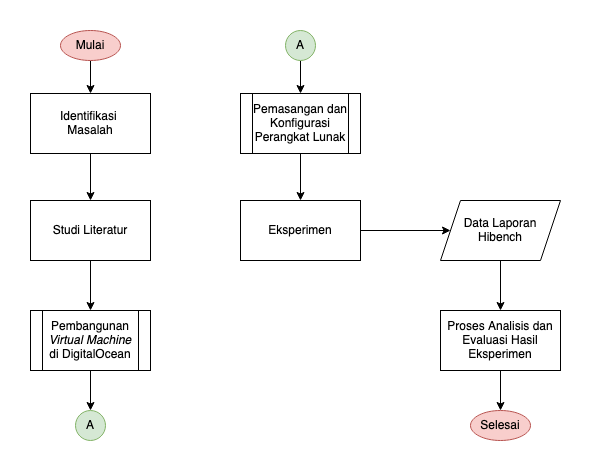
\includegraphics[width=0.85\textwidth]{figures/ch03/Diagram Tugas Akhir.png}
    \caption{Diagram Alir Penelitian}
    \label{fig:diagram alir}
\end{figure}

\section{Membangun \textit{Virtual Machine} di DigitalOcean}
Konfigurasi perangkat keras merupakan aspek penting dalam mengevaluasi kinerja aplikasi \textit{big data} berbasis Hadoop dan Spark. Penelitian ini memerlukan penggunaan mesin virtual, Droplets pada DigitalOcean, yang memungkinkan untuk menyesuaikan berbagai aspek seperti sistem operasi, kapasitas penyimpanan, jumlah prosesor, dan parameter lainnya sesuai dengan kebutuhan spesifik penelitian.

Penelitian ini mengadopsi mode \textit{pseudo-distributed} yang memungkinkan penggunaan hanya satu \textit{virtual machine} dalam konfigurasi \textit{single node}. Walaupun hanya menggunakan satu \textit{virtual machine}, mode \textit{pseudo-distributed} memungkinkan setiap proses dalam klaster beroperasi secara independen, menciptakan lingkungan di mana semua proses berjalan mandiri satu sama lain. Hal ini memungkinkan untuk lebih berfokus pada pengumpulan data dan analisis, tanpa perlu melakukan konfigurasi yang rumit terkait dengan pengaturan klaster. Spesifikasi perangkat keras yang digunakan untuk \textit{virtual machine} dalam mode \textit{pseudo-distributed} sesuai pada Tabel \ref{table:conf-hardware}. Penjelasan lengkap tentang pembuatan \textit{virtual machine} (VM) pada \textit{platform} DigitalOcean dan cara mengakses VM tersebut disajikan pada Lampiran \ref{appendix:A}.

\begin{table}[h]
	\centering
	\caption{Konfigurasi Perangkat Keras}
	\begin{tabular}{l p{9cm}} 
		\toprule
		\textbf{Nama Parameter}    & \textbf{Nilai Parameter} \\ 
        \midrule
		\textbf{Lokasi Pusat Data} & Singapore - Datacenter 1 - SGP1               \\ 
		\textbf{Sistem Operasi}    & Ubuntu 20.04 (LTS) x64                        \\
		\textbf{Jenis \textit{Droplet}}     & Basic                                         \\ 
		\textbf{Prosesor}          & Premium AMD - 4 Core                          \\ 
		\textbf{Memori}            & 8 GB                                          \\ 
		\textbf{Penyimpanan}       & 160 GB NVMe SSD                               \\ 
        \bottomrule
	\end{tabular}
	\label{table:conf-hardware}
\end{table}

\section{Pemasangan dan Konfigurasi Perangkat Lunak}
Pemasangan dan konfigurasi perangkat lunak merupakan hal yang krusial dalam penelitian ini. Perangkat lunak yang diperlukan ditunjukkan pada Tabel \ref{table:software-needs}. Selanjutnya, alur instalasi perangkat lunak dalam penelitian ini dapat dilihat pada Gambar \ref{fig:alurkerja-soft}. Terdapat tiga bagian utama, yaitu \textit{prerequisites} (perangkat lunak prasyarat) ditandai dengan warna biru, alat penyimpanan dan pemrosesan \textit{Big Data} ditandai dengan warna jingga, dan alat untuk mengukur kinerja \textit{big data} ditandai dengan warna hijau. 

\begin{table}[h!]
	\centering
	\caption{Perangkat Lunak yang Dibutuhkan}
		\begin{tabular}{l p{9cm}} 
		\toprule
			\textbf{Perangkat Lunak} & {\textbf{Deskripsi}}\\ 
            \midrule
			Ubuntu 20.04 LTS x64     & Sistem operasi Linux berbasis Ubuntu  \\ 
			Git                      & Sistem kontrol versi  \\
			Maven                    & Perangkat lunak manajemen proyek Java                            \\ 
			Java 8                   & Bahasa pemrograman                                 \\ 
			Python 3.7               &  Bahasa pemrograman                                                                                                                      \\
			Scala 2.11.8               & Bahasa pemrograman                                                                                                                       \\
			Hadoop 2.4                & Perangkat lunak \textit{big data}\\ 
			Spark 2.1.3               & Perangkat lunak \textit{big data} \\ 
			Hibench   & Alat mengukur kinerja Hadoop dan Spark                                                            \\
			Dool   & Alat melihat penggunaan \textit{resource} sistem                                                             \\
            \bottomrule 
		\end{tabular}
	\label{table:software-needs}
\end{table}

%\begin{landscape}
%\begin{figure}
%    \centering
%    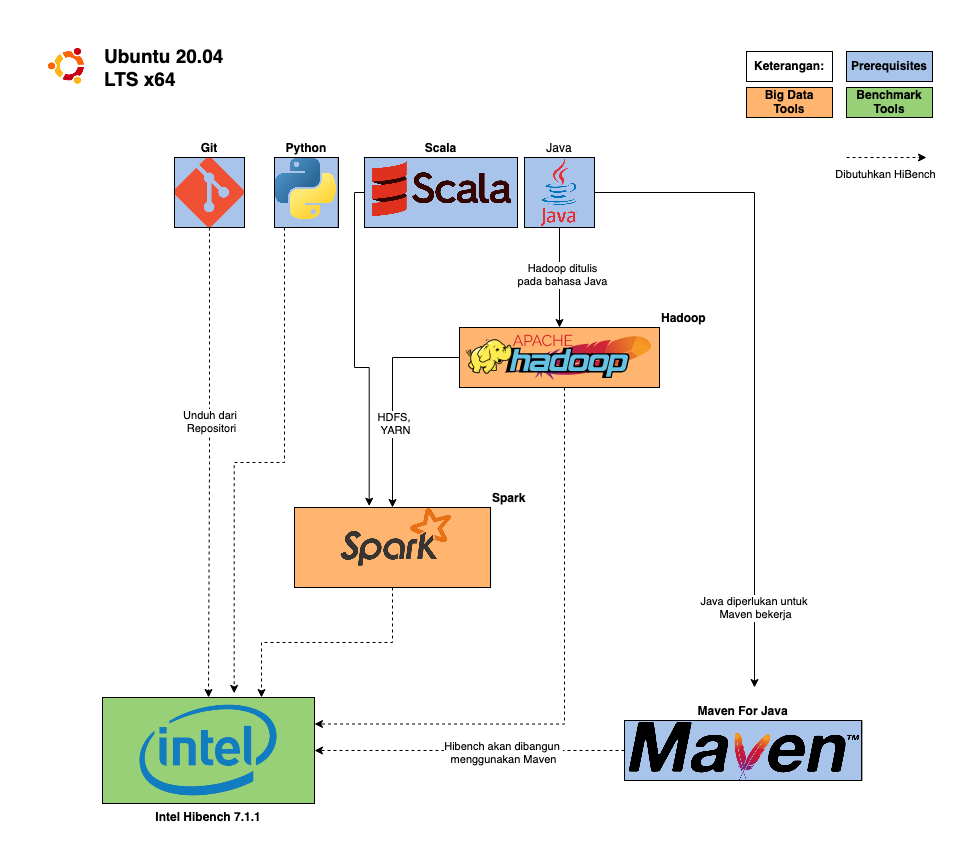
\includegraphics[height=0.6\linewidth]{figures/ch03/alurkerja-soft.png}
%    \caption{Alur Instalasi Perangkat Lunak}
%    \label{fig:alurkerja-soft}
%\end{figure}
%\end{landscape}

\subsection{Instalasi Perangkat Lunak Prasyarat}
Ada beberapa perangkat lunak yang perlu dipasang sebelum menggunakan Hadoop, Spark, dan HiBench, yaitu Ubuntu 20.04 LTS x64, Git, Java 8 dan Maven, Python 3.7, dan Scala 2.11.8. Pemasangan dan konfigurasi perangkat lunak pada tahapan ini tidak membutuhkan urutan. Akan tetapi, pada penelitian ini dibuatkan alur untuk pemasangan dan konfigurasi perangkat lunak prasyarat seperti pada Gambar \ref{fig:prasyarat-flow}. Penjelasan lebih lengkap mengenai tata cara instalasi dan konfigurasi perangkat lunak prasyarat ini disajikan pada Lampiran \ref{appendix:B}. 

\begin{figure}[h!]
    \centering
    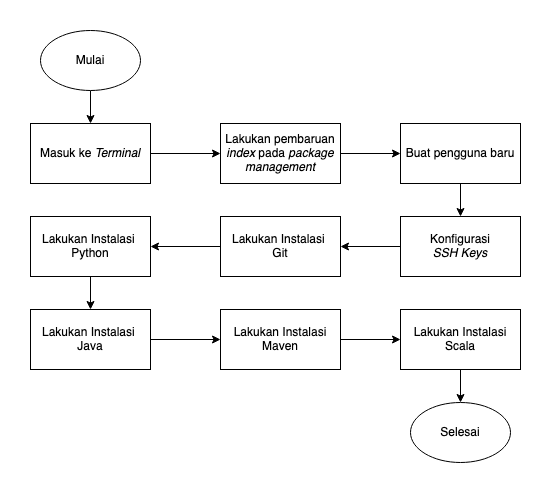
\includegraphics[width=0.75\textwidth]{figures/ch03/prasayarat-flow.png}
    \caption{Alur Instalasi Perangkat Lunak Prasyarat}
    \label{fig:prasyarat-flow}
\end{figure}

\begin{landscape}
\begin{figure}
    \centering
    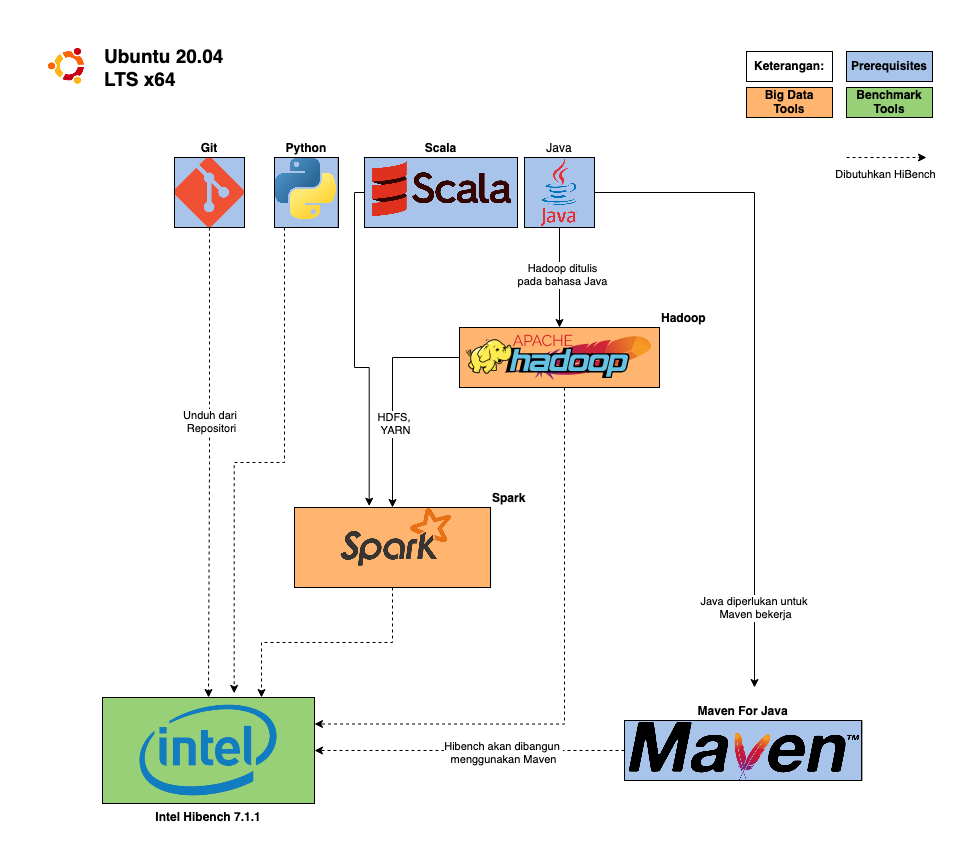
\includegraphics[height=0.6\linewidth]{figures/ch03/alurkerja-soft.png}
    \caption{Alur Instalasi Perangkat Lunak}
    \label{fig:alurkerja-soft}
\end{figure}
\end{landscape}

\subsection{Instalasi dan Konfigurasi Hadoop}
Hadoop adalah perangkat lunak \textit{open source} yang efektif dalam menyimpan dan memproses data dalam skala besar. Hadoop memungkinkan pengklasteran beberapa komputer untuk menganalisis  data besar secara paralel dengan lebih cepat. Setelah perangkat lunak prasyarat berhasil dipasang, Hadoop dapat dipasang mengikuti panduan lengkap pada Lampiran \ref{appendix:C}. Konfigurasi Hadoop supaya dapat berjalan pada \textit{pseudo distributed} meliputi pengubahan kepemilikian berkas Hadoop, mematikan fitur IPv6, menambahakan Hadoop pada \textit{env}, dan mengatur konfigurasi komponen Hadoop sesuai dengan Gambar \ref{fig:hadoop-flow}.

\begin{figure}[h!]
    \centering
    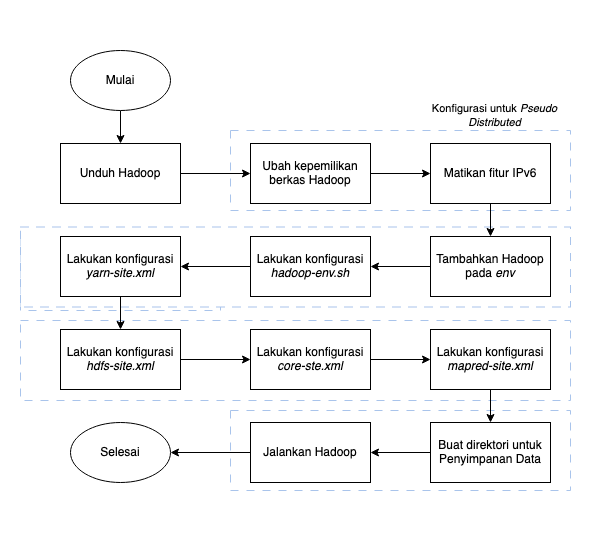
\includegraphics[width=0.9\textwidth]{figures/ch03/hadoop-flow.png}
    \caption{Alur Instalasi dan Konfigurasi Hadoop}
    \label{fig:hadoop-flow}
\end{figure}

\subsection{Instalasi dan Konfigurasi Spark}
Spark dan Hadoop memiliki hubungan yang erat. Spark dapat berjalan di \textit{Hadoop Distributed File System} (HDFS) dan dapat menggunakan Hadoop YARN sebagai manajer sumber daya. Oleh karena itu, instalasi Spark membutuhkan Hadoop terpasang lebih dahulu. Alur pemasangan dan konfigurasi spark terlihat seperti pada Gambar \ref{fig:spark-flow}. Apabila Hadoop sudah berhasil terpasang, langkah selanjutnya adalah memasang Spark seperti pada Lampiran \ref{appendix:D}.

\begin{figure}[h]
    \centering
    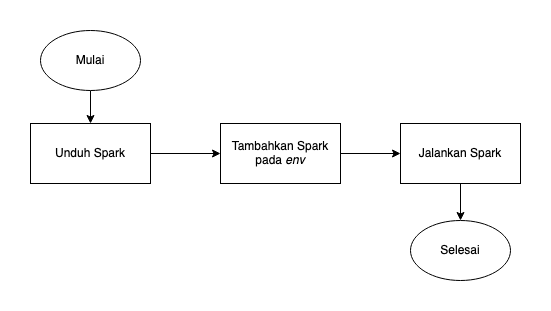
\includegraphics[width=0.8\textwidth]{figures/ch03/spark-flow.png}
    \caption{Alur Instalasi dan Konfigurasi Spark}
    \label{fig:spark-flow}
\end{figure}

\subsection{Instalasi dan Konfigurasi HiBench}
Sebelum melakukan eksperimen, diperlukan suatu perangkat lunak pengukuran kinerja sistem \textit{Big Data}, yaitu HiBench. HiBench tidak dapat digunakan secara langsung ketika sudah berhasil diunduh, melainkan harus dilakukan pembangunan beberapa modul yang dibutuhkan dengan Maven dan konfigurasi beberapa parameter. 

Secara umum, alur instalasi dan konfigurasi HiBench sesuai dengan Gambar \ref{fig:hibench-flow}. Berkas HiBench diunduh dari repositori, dilanjutkan dengan pembangunan beberapa modul yang nantinya dibutuhkan. Selanjutnya, dilakukan konfigurasi beberapa berkas seperti \textit{hibench.conf}, hadoop.conf, dan spark.conf. Jika telah dilakukan konfigurasi, dapat dilanjutkan dengan menjalankan beban kerja atau eksperimen. Lebih lanjut, pemasangan dan konfigurasi HiBench dijelaskan pada Lampiran \ref{appendix:E}.

\begin{figure}[h]
    \centering
    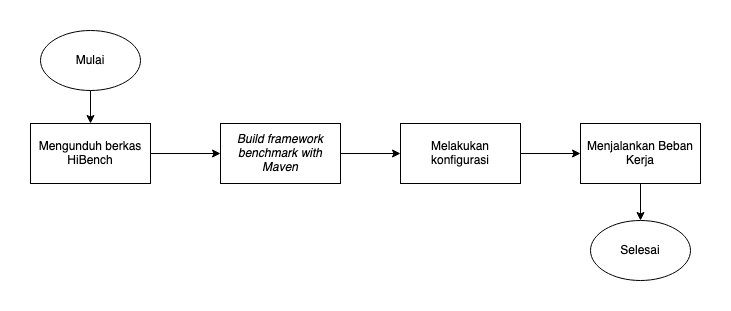
\includegraphics[width=1\textwidth]{figures/ch03/hibench-flow.png}
    \caption{Alur Instalasi dan Konfigurasi HiBench}
    \label{fig:hibench-flow}
\end{figure}

%\begin{table}[]
%\caption{Konfigurasi \textit{HiBench}}
%\label{table:conf-hibench}
%\scriptsize
%\centering
%\begin{tabular}{ll}
%\hline
%\multicolumn{1}{c}{Nama Parameter}  & \multicolumn{1}{c}{Nilai} \\ \hline
%hibench.default.map.parallelism     & 8                         \\
%hibench.default.shuffle.parallelism & 8 \\ \hline                        
%\end{tabular}
%\end{table}


\section{Eksperimen}
Setelah instalasi dan konfigurasi perangkat keras dan perangkat lunak berhasil diselesaikan, tahap selanjutnya adalah eksperimen. Tahap ini melibatkan serangkaian pengujian yang terkontrol untuk mengevaluasi kinerja \textit{platform big data} Hadoop dan Spark dalam menjalankan beban kerja tertentu dengan berbagai ukuran data. Tujuan utama eksperimen ini adalah untuk menjawab pertanyaan penelitian yang telah didefinisikan sebelumnya dan memperoleh pemahaman yang komprehensif tentang karakteristik kinerja masing-masing \textit{platform}.

Penelitian ini difokuskan pada pengujian dua beban kerja yang umum dalam pemrosesan big data, yaitu \textit{word count} dan \textit{sort}. Beban kerja ini akan dieksekusi pada dua \textit{platform big data} yang populer, yaitu Hadoop dan Spark. Setiap kombinasi \textit{platform} dan beban kerja akan diuji dengan 12 ukuran data yang berbeda, mulai dari 100 KB hingga 15 GB. Detail ukuran data yang digunakan ditunjukkan pada Tabel \ref{table:variasi-input-data}. Untuk memastikan reliabilitas dan konsistensi hasil, setiap kombinasi \textit{platform}, beban kerja, dan ukuran data akan diulang sebanyak lima kali. 

Proses eksperimen menghasilkan dua jenis berkas data: 
\begin{enumerate}
	\item \textit{HiBench Report}: Berisi informasi tentang kinerja beban kerja, termasuk waktu eksekusi, dan \textit{throughput}.
	\item \textit{Dool System Monitoring}: Berisi informasi detail tentang aktivitas sistem selama eksekusi beban kerja, seperti penggunaan CPU, memori, I/O \textit{disk}, dan jaringan.
\end{enumerate}

Secara keseluruhan, desain eksperimen ini menghasilkan 240 percobaan individu. Setiap percobaan mewakili kombinasi unik dari:
\begin{enumerate}
	\item \textit{Platform big data} (Hadoop atau Spark)
	\item Beban kerja (\textit{word count} atau \textit{sort})
	\item Ukuran data (12 variasi)
	\item Pengulangan (lima kali)
\end{enumerate}

%\begin{figure}[h]
%    \centering
%    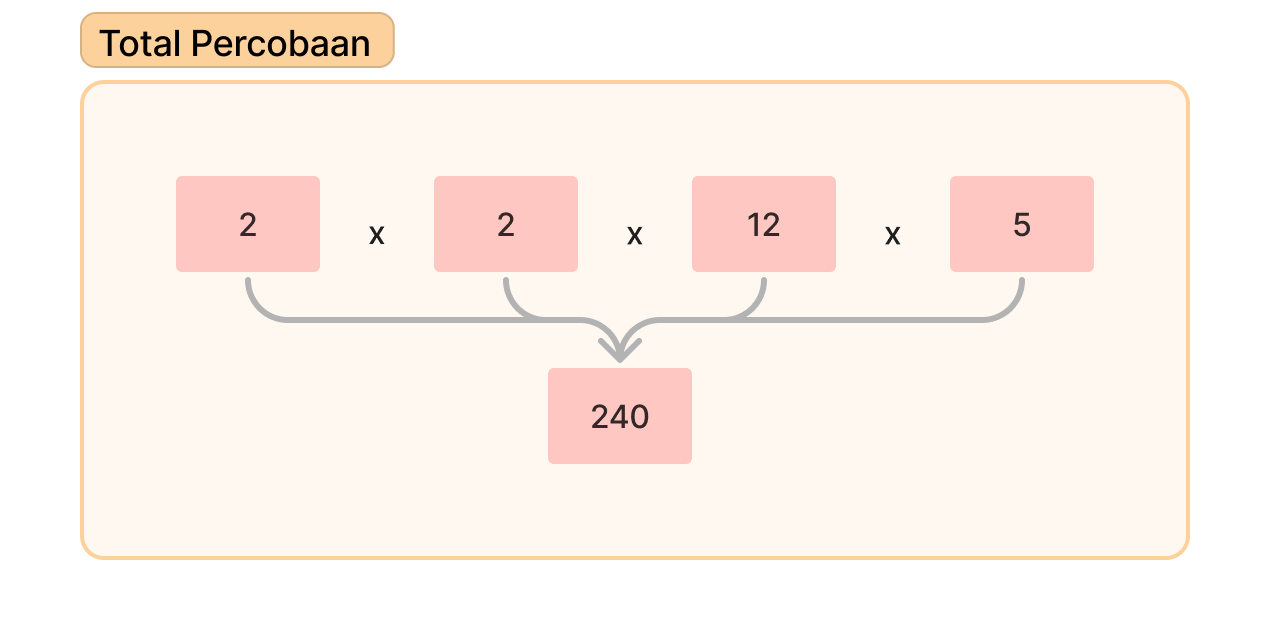
\includegraphics[width=0.7\textwidth]{figures/ch03/total-percobaan.png}
%    \caption{Total Percobaan}
%    \label{fig:total-percobaan}
%\end{figure}

\begin{landscape}
\begin{figure}[h]
    \centering
    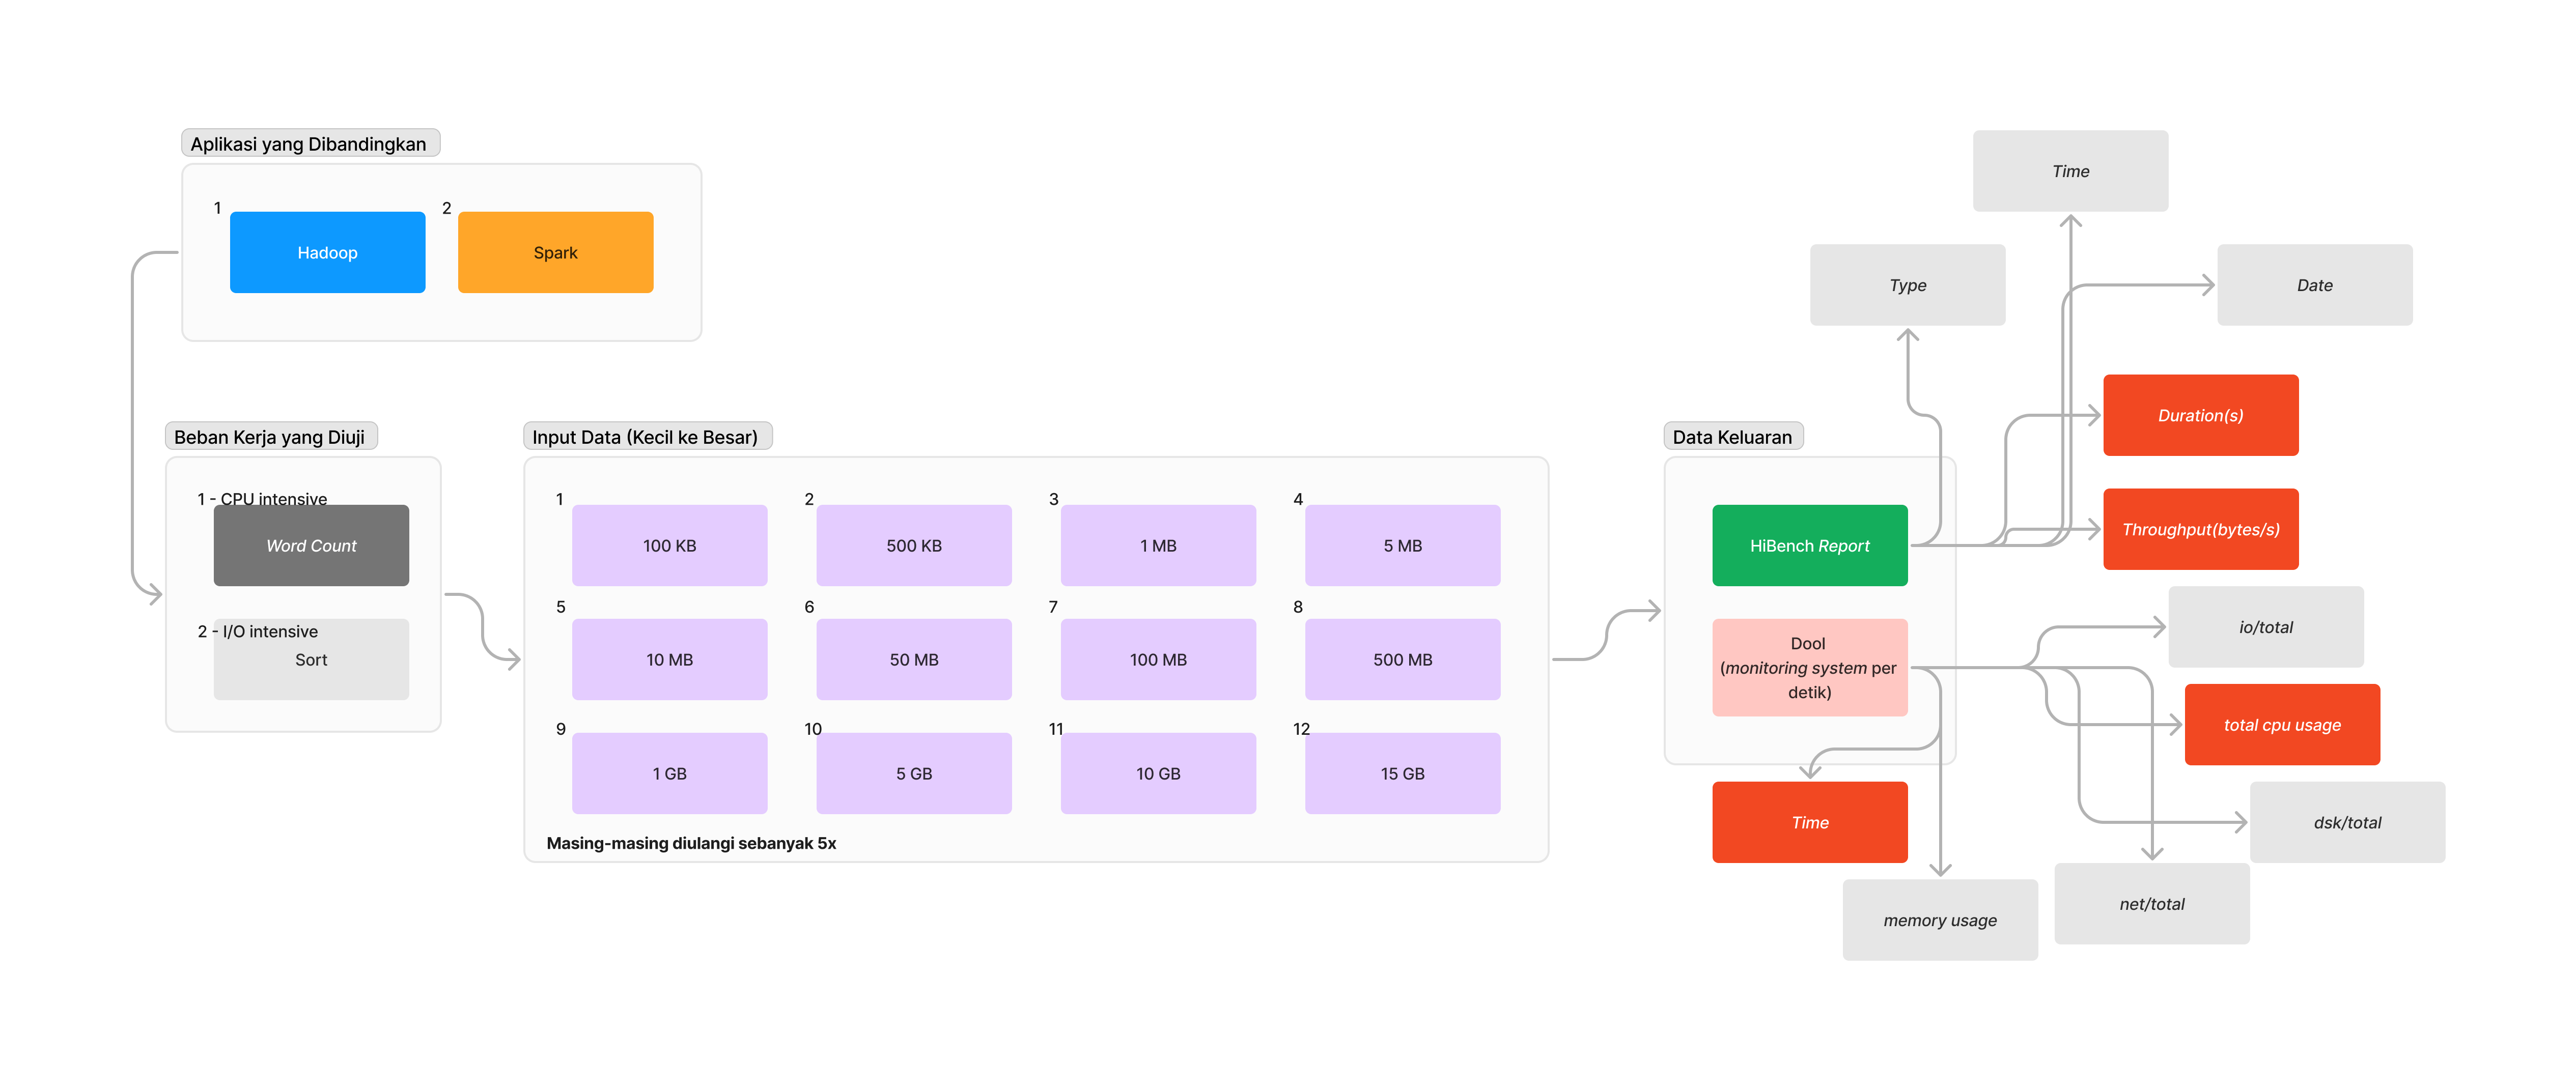
\includegraphics[width=\linewidth, height=0.5\linewidth]{figures/ch03/flow-penelitian-umum.png}
    \caption{\textit{End-to-end} Penelitian}
    \label{fig:flow-penelitian-umum}
\end{figure}
\end{landscape}

Sebagai contoh, \textit{platform} Hadoop dengan beban kerja \textit{word count} dan ukuran data 100 KB, akan menghasilkan lima HiBench \textit{Report} dan lima berkas Dool \textit{System Monitoring}, sesuai dengan jumlah pengulangan.  Ilustrasi ini dapat dilihat pada Gambar \ref{fig:contoh-percobaan}.

\begin{figure}[h]
    \centering
    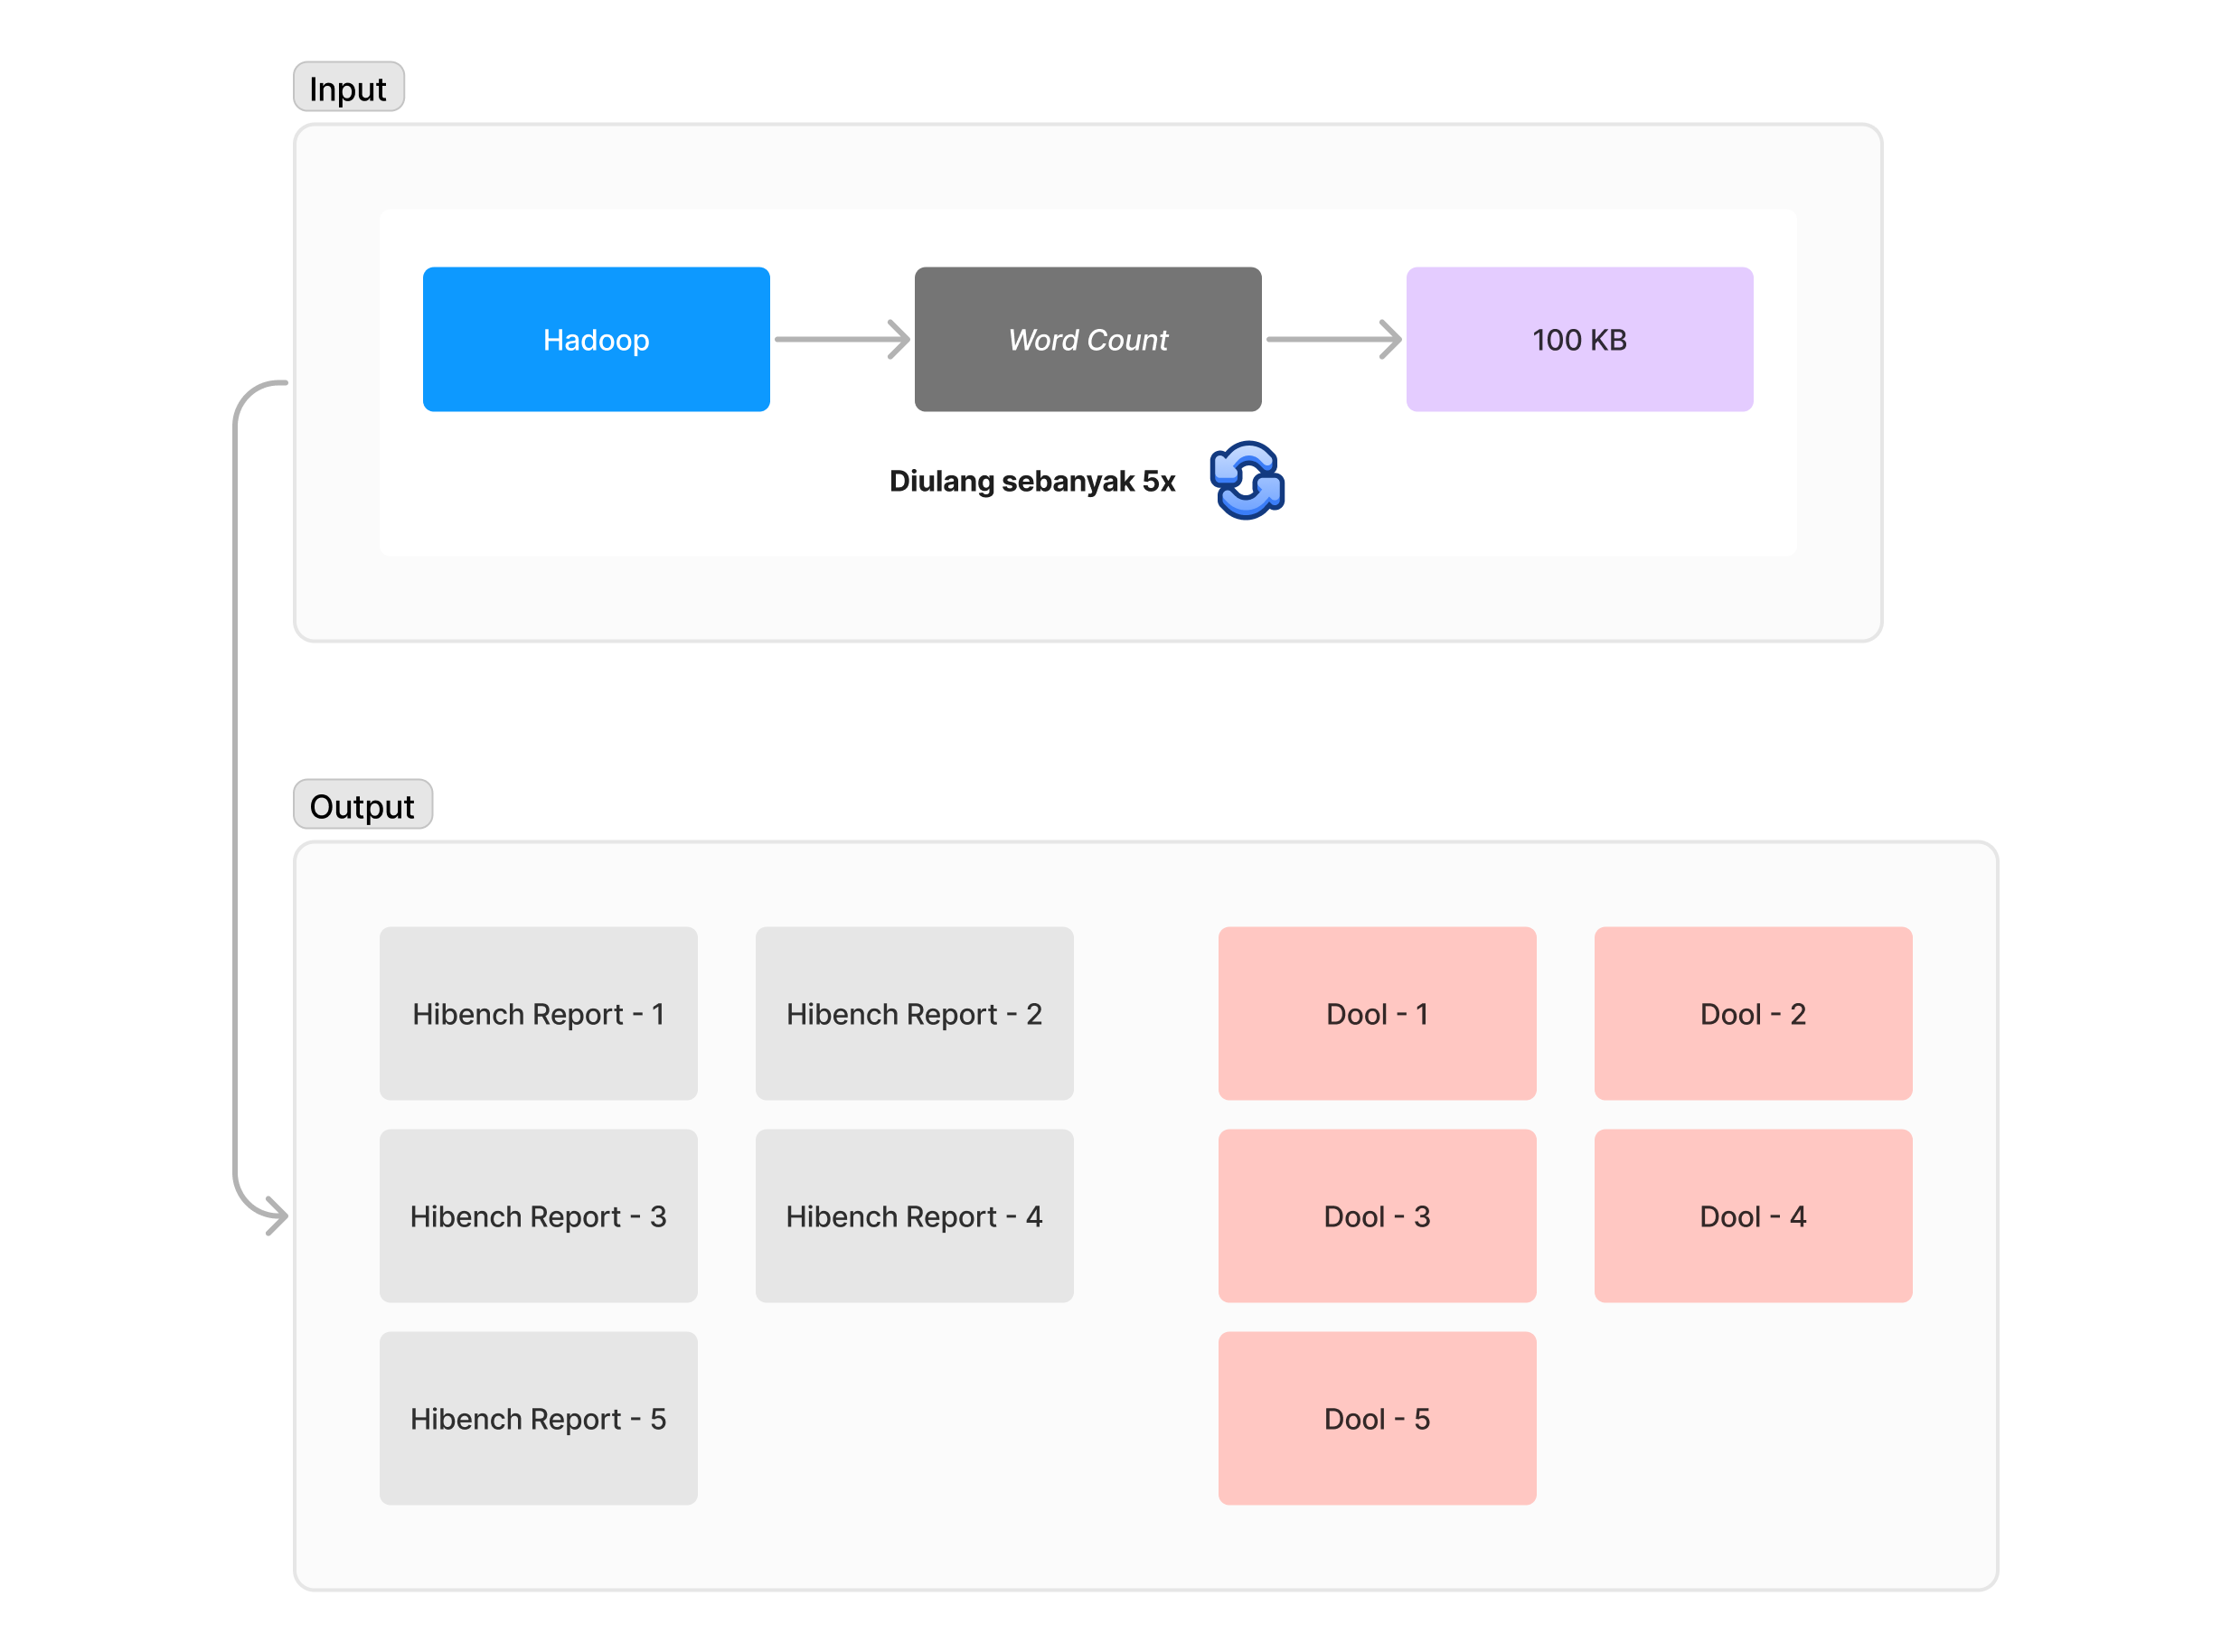
\includegraphics[width=0.9\textwidth]{figures/ch03/contoh-percobaan.png}
    \caption{Contoh Percobaan}
    \label{fig:contoh-percobaan}
\end{figure}

\begin{table}[]
\caption{Variasi Input Data}
\label{table:variasi-input-data}
\centering
\begin{tabular}{lll}
\hline
\multicolumn{1}{c}{\textbf{Label Input Data}} & \multicolumn{1}{c}{\begin{tabular}[c]{@{}c@{}}\textbf{Ukuran Input Data  (bita)}\end{tabular}} \\ \hline
100 KB & 100000 ($1 x 10^5$) \\
500 KB & 500000 ($5 x 10^5$) \\
1 MB   & $1 x 10^6$          \\
5 MB   & $5 x 10^6$          \\
10 MB  & $1 x 10^7$          \\
50 MB  & $5 x 10^7$          \\
100 MB & $1 x 10^8$          \\
500 MB & $5 x 10^8$          \\
1 GB   & $1 x 10^9$          \\
5 GB   & $5 x 10^9$          \\
10 GB  & $1 x 10^{10}$         \\ 
15 GB  & $1.5 x 10^{10}$       \\ \hline
\end{tabular}
\end{table}


Otomatisasi menjadi penting untuk memastikan efisiensi dan akurasi karena jumlah percobaan yang banyak. Skrip otomatisasi dikembangkan untuk mengotomatiskan seluruh proses eksperimen. Detail skrip otomatisasi dapat ditemukan pada Lampiran \ref{appendix:F}.

Algoritma otomatisasi eksperimen dimulai dengan mengubah direktori kerja ke direktori HiBench.  Selanjutnya, algoritma melakukan iterasi untuk setiap beban kerja yang ditentukan.  Di dalam setiap iterasi beban kerja, dilakukan iterasi lagi untuk setiap ukuran data.  Pada setiap kombinasi beban kerja dan ukuran data, konfigurasi HiBench diubah sesuai dengan ukuran data yang dipilih.

Skrip persiapan data Hadoop dan Spark dijalankan sebelum eksekusi beban kerja dilakukan. Setelah data siap, eksekusi beban kerja akan dijalankan. Setiap perulangan, perangkat lunak \textit{Dool} dijalankan untuk memonitor aktivitas sistem. Setelah semua perulangan selesai, algoritma menunggu selama 15 detik sebelum melanjutkan ke ukuran data berikutnya. Proses ini berlanjut hingga semua kombinasi beban kerja dan ukuran data selesai diproses.

\section{Analisis dan Evaluasi Hasil Eksperimen}

Setelah menyelesaikan 240 percobaan yang dijelaskan di bagian eksperimen, langkah selanjutnya adalah menganalisis dan mengevaluasi hasil yang diperoleh. Analisis ini bertujuan untuk menjawab pertanyaan penelitian dan memahami bagaimana kinerja Hadoop dan Spark dalam menjalankan beban kerja \textit{word count} dan \textit{sort} dengan berbagai ukuran data. Berikut adalah beberapa aspek yang akan dikaji:

\begin{enumerate}	
	\item \textbf{Kinerja}
	\begin{enumerate}
		\item Persebaran Waktu Eksekusi pada Hadoop dan Spark. Bagian ini akan menganalisis sebaran waktu eksekusi untuk setiap beban kerja (\textit{word count} dan \textit{sort}) pada kedua aplikasi (Hadoop dan Spark) dengan berbagai ukuran data. Analisis ini akan membantu memahami variabilitas kinerja dan konsistensi hasil pada setiap kombinasi aplikasi, beban kerja, dan ukuran data.
		\item Persebaran \textit{Throughput} pada Hadoop dan Spark. Mirip dengan analisis waktu eksekusi, persebaran \textit{throughput} juga akan dianalisis untuk setiap kombinasi aplikasi, beban kerja, dan ukuran data. Throughput, yang menunjukkan jumlah data yang diproses per satuan waktu,  merupakan metrik penting dalam evaluasi kinerja sistem \textit{big data}.  Visualisasi distribusi \textit{throughput} akan membantu dalam memahami efisiensi pemrosesan data oleh Hadoop dan Spark.
	\end{enumerate}
	\newpage
	\item \textbf{Penggunaan Sumber Daya}
	\begin{enumerate}
	\item Penggunaan CPU. Bagian ini akan menganalisis penggunaan CPU oleh Hadoop dan Spark selama menjalankan berbagai beban kerja.  Informasi ini dapat diperoleh dari berkas \textit{monitoring} sistem yang dihasilkan oleh Dool.  Analisis penggunaan CPU membantu memahami bagaimana setiap \textit{platform} memanfaatkan sumber daya komputasi dan mengidentifikasi potensi optimasi.
	\item Utilisasi Sistem. Selain penggunaan CPU, metrik-metrik lain seperti penggunaan memori, dan I/O penyimpanan. Hal ini memberikan gambaran yang lebih komprehensif tentang bagaimana setiap \textit{platform} memanfaatkan sumber daya sistem dan potensi \textit{bottleneck} yang mungkin terjadi selama pemrosesan data besar.
	\end{enumerate}
\end{enumerate}











